% vim: ai sw=2 spell spelllang=en

\documentclass[xcolor=dvipsnames]{beamer}

\let\Oldemph\emph
\renewcommand{\emph}[1]{\textcolor{blue}{\Oldemph{#1}}}
\newcommand{\heading}[1]{\textbf{\textcolor{BurntOrange}{#1}}}
\newcommand{\header}[1]{\textbf{\texttt{\textcolor{WildStrawberry}{#1}}}}
\newcommand{\doc}[1]{\textbf{\texttt{\textcolor{OliveGreen}{#1}}}}

\newcommand{\cdb}{\textbf{\textsc{ClabureDB}}\xspace}
\newcommand{\klee}{\textsc{Klee}\xspace}
\newcommand{\stan}{\textbf{\textsc{Stanse}}\xspace}
\newcommand{\symb}{\textbf{\textsc{Symbiotic}}\xspace}

\mode<presentation>
{
\usetheme{Madrid}
}

\setbeamertemplate{navigation symbols}{}
\setbeamertemplate{footline}[frame number]{}

\usepackage{adjustbox}
\usepackage[utf8x]{inputenc}
\usepackage{helvet}
\usepackage{mathptmx}
\usepackage[IL2]{fontenc}
\usepackage{graphicx}
\usepackage{hyperref}
\usepackage[final]{listings}
\usepackage{multirow}
\usepackage{tikz}
\usepackage[absolute,overlay]{textpos}
\usepackage{xspace}
\usetikzlibrary{arrows, positioning}

\tikzset{tl_state/.style={rounded corners, thick, draw, minimum height=6mm,
	minimum width=12mm, bottom color=black!15, top color=black!5}}
\tikzset{tl_phase/.style={thick, draw, minimum size=8mm}}
\tikzset{tl_edge/.style={<-, >=stealth', semithick}}

\lstset{tabsize=2,numbers=none,showstringspaces=false,breaklines=true,
	breakatwhitespace=true,escapeinside={(*@}{@*)},
	basicstyle=\scriptsize,keywordstyle=\bfseries\color{OliveGreen},
	commentstyle=\color{blue}, columns=flexible, language=C}

\newcommand{\cmd}[2][]{\lstinline[columns=fullflexible, language=bash,
	basicstyle=\ttfamily, #1]$#2$}
\newcommand{\code}[2][]{\lstinline[columns=fullflexible, basicstyle=\ttfamily,
	#1]$#2$}

\title{Automatic Bug-finding Techniques \\ for Large Software Projects}
\subtitle{Ph.D. Thesis}
\date{March 4\textsuperscript{th} 2014, Brno}

\author{Jiri~Slaby}

\institute{Faculty of Informatics\\
Masaryk University}

\begin{document}

\begin{frame}
  \titlepage
\end{frame}

%%%%%%%%%%%%%%%%%%%%%%%

\begin{frame}
  \frametitle{Presentation Outline}
  \begin{itemize}
    \item Introduction

    \pause

    \item Thesis Contribution
    \begin{itemize}
      \item Publications and Software
      \item Competition
    \end{itemize}

    \pause

    \item Conclusion
  \end{itemize}

\end{frame}

\begin{frame}
  \frametitle{Motivation}
% U slajdu 3 bych zminl (jen slovne, ne na slajd), ze ta suma i procento budou
% patrne za tech 12 let o neco vyssi.

  \begin{center}
    \Large{Software Errors Cost U.S. Economy}\\[1.3ex]
    \textbf{\LARGE\$59.5 Billion}\\[1ex]
    \Large{Annually}\\[4ex]

    \small{0,6 Percent of the Gross Domestic Product}\\[1ex]

    \scriptsize{(2002, US study)}
  \end{center}

\end{frame}

\begin{frame}
  \frametitle{Analyzing Large Projects}
%A rozebrat, ktere metody se hodi min/vic.  Zejmena zduraznit nutnost plne
%automatizace a vysoke presnosti vysledku.  Zduraznit, jak nesnadny je to ukol.

  \heading{Large Projects}
  \begin{itemize}
    \item \textbf{Aim of the thesis}

    \pause

    \item They are special when analyzed
    \begin{itemize}
      \item Millions lines of \emph{complex} code
      \item Resources needed (computational time, memory, \dots)
      \item Diverse kinds of errors
      \item Language mixture and dialects
      \item Manual annotations are hard
    \end{itemize}

    \pause

    \item All our techniques exercised on the Linux kernel
  \end{itemize}

\end{frame}

\begin{frame}
  \frametitle{Program Analysis}

  \heading{Program Analysis}
  \begin{itemize}
    \item Use: \emph{finding errors}, optimizations, reverse engineering, \dots

    \pause

    \item Two main kinds
    \begin{enumerate}
      \item Dynamic analysis
      \begin{itemize}
	\item Run on a processor and inspect (e.g.\ testing)
	\item \textbf{Out of scope for this thesis}
      \end{itemize}

      \pause

      \item Static analysis
      \begin{itemize}
	\item \textbf{Aim of this thesis}
      \end{itemize}
    \end{enumerate}
  \end{itemize}

\end{frame}

\begin{frame}
  \frametitle{Static Analysis}

  \begin{center}
    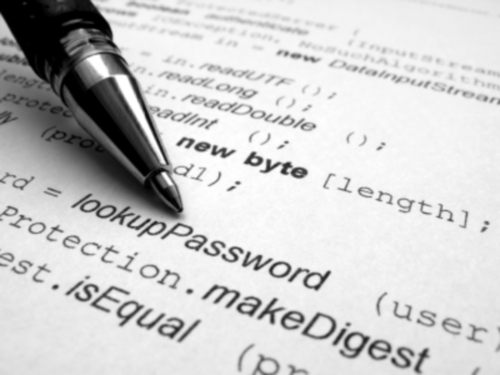
\includegraphics{why-static-analysis}\\
    \tiny{Source: plynt.com}
  \end{center}

  \begin{center}
    \Large
    \heading{Static analysis}\\[0.7ex]
      In our understanding\\
      the term static analysis means analyzing code\\
      without directly executing it on a processor.
  \end{center}

\end{frame}

\begin{frame}
  \frametitle{Thesis Contribution}

  \heading{Contribution: Publications and Software}
  \begin{enumerate}
    \item Tuning Abstract interpretation in \stan
    \item New approach to Symbolic execution in \symb
    \item Static analyzers testbed as \cdb
    \item Competition and \symb
  \end{enumerate}

%  \pause
%  \bigskip
%
%  \begin{center}
%    \heading{All tested on the Linux kernel}
%  \end{center}

\end{frame}

\begin{frame}
  \frametitle{\stan}

  \begin{itemize}
    \item Employs
    \begin{itemize}
      \item Abstract interpretation
      \item Statistical lock checking
      \item Locksets
      \item Graph reachability
    \end{itemize}

    \pause

    \item No real contribution to the \emph{theory} of the techniques

    \pause

    \item Highly optimized to large projects
    \begin{itemize}
      \item Fast parsing (build system support, optimized parser, streaming)
      \item Language-indepentent pattern matching
      \item Reduced false alarms (tuned detectors, filters)
      \item Optimized and fast analyses
      \item And more\dots
    \end{itemize}
  \end{itemize}

  \smallskip
  \pause

  \begin{center}
    \heading{When all that was glued together,\\
    \stan found over 170 errors in the kernel,\\
    all confirmed later.}
  \end{center}

\end{frame}

\defverbatim{\lstone}{%
  \begin{lstlisting}
sss
  \end{lstlisting}}

\begin{frame}[fragile]
  \frametitle{Symbolic Execution for Large Projects}

  \begin{itemize}
    \item<1-> \stan still reports \emph{false alarms}

    \item<2-> We invented a technique using the Symbolic execution
    \begin{itemize}
      \item More precise approach
      \item But slower
    \end{itemize}

    \item<3-> Fitting large projects in 3 steps
    \begin{enumerate}
      \item<4-> Automatically instrument -- add properties
      \item<5-> Slice -- leave only relevant code (\emph{real speedup})
      \item<6-> Symbolically execute -- more precise error finding
    \end{enumerate}

    \item<7-> Implemented in \symb
  \end{itemize}

  \begin{center}
  \begin{semiverbatim}
    \only<3-5>{\alert<5>{lock(A);}}\only<6->{        }   \only<4->{\alert<4>{fire(get_automaton(A), LOCK);}}
    \only<3-5>{\alert<5>{while (to_compute())}}
    \only<3-5>{\alert<5>{  compute();}}
    \only<3-5>{\alert<5>{unlock(A);}}\only<6->{          } \only<4->{\alert<4>{fire(get_automaton(A), UNLOCK);}}
  \end{semiverbatim}
  \end{center}

\end{frame}

\begin{frame}[fragile]
  \frametitle{\cdb}

  \begin{textblock*}{4cm}(8.7cm,1cm)
  \only<2->{
    \includegraphics[width=\textwidth]{error}
  }
  \end{textblock*}

  \heading{Database for evaluation of bug-finding tools}
  \begin{itemize}
    \item Questions
    \begin{itemize}
      \item Did the tool find all real errors?
      \item How many false alarms did it report?
    \end{itemize}

    \pause

    \item \cdb is the answer
    \begin{itemize}
      \item Instantly: no manual sorting
    \end{itemize}

    \pause

    \item Three projects (the Linux kernel inclusive)

    \pause

    \item Thousands of found errors in the projects
    \begin{itemize}
      \item Seven sources
      \item Most errors are classified as \textit{real error} or
        \textit{false alarm}
    \end{itemize}

  \end{itemize}

  \smallskip

  \begin{center}
  \Large
  \url{http://claburedb.fi.muni.cz/}
  \end{center}

\end{frame}

\begin{frame}
  \frametitle{SV-COMP}

  \heading{Competition on Software Verification}
  \begin{itemize}
    \item Program analyzers compete
    \begin{itemize}
      \item About 10 categories, 15 tools
    \end{itemize}

    \pause

    \item We participated twice
    \begin{itemize}
      \item We were on 4th and 5th places in several categories
      \item It helps us to improve \symb significantly
    \end{itemize}
  \end{itemize}

\end{frame}

\begin{frame}
  \frametitle{Conclusion}

  \heading{Direction of Static Analyzers}
  \begin{itemize}
    \item Handle more code (faster analyses)
    \item Better accuracy = less false alarms
  \end{itemize}

  \bigskip
  \bigskip

  \begin{center}
    \large
    \heading{We contributed to this goal}
  \end{center}

\end{frame}

\begin{frame}
  \frametitle{Activity Summary}

  \begin{itemize}
    \item Thesis publications
    \begin{enumerate}
      \small
      \item J. Slaby, J. Strejček. Symbiotic 2: More Precise Slicing. TACAS.
      Springer, 2014. (\emph{To appear.})

      \item J. Slaby, J. Strejček, and M. Trtík. Symbiotic: Synergy of
      instrumentation, slicing, and symbolic execution. TACAS. Springer, 2013.

      \item J. Slaby, J. Strejček, and M. Trtík. ClabureDB: Classified
      bug-reports database. VMCAI. Springer, 2013.

      \item J. Slaby, J. Strejček, and M. Trtík. Checking properties
      described by state machines: On synergy of instrumentation, slicing, and
      symbolic execution. FMICS. Springer, 2012.

      \item J. Obdržálek, J. Slabý, and M. Trtík. STANSE: Bug-finding framework
      for C programs. MEMICS. Springer, 2011.

    \end{enumerate}

    \item Other publications: 3
    \item Software: \stan, \symb, \cdb
    \item Teaching: advanced C courses (Linux kernel, Low-level Linux)
    \item Lead theses: 5 (2 more to appear)
  \end{itemize}

\end{frame}

\appendix
\newcounter{finalframe}
\setcounter{finalframe}{\value{framenumber}}

\begin{frame}
  \frametitle{Abstract Interpretation in \stan}

  \begin{center}
  \begin{tabular}{cp{1em}c}
    \tikzstyle{stat} = [circle,thick,draw,minimum size=8mm]
    \tikzstyle{edge} = [shorten <=1pt,>=stealth',semithick]
    \adjustbox{valign=m}{\scalebox{0.7}{
    \begin{tikzpicture}[node distance=18mm,font=\sffamily]

      \node [stat] (ERR) {\textbf{Err}}
	edge [edge,loop above] node[right, xshift=2mm, yshift=-2mm]
	  {\code{lock()}/\code{unlock()}} ();

      \node [stat] (U) [below left=of ERR] {U}
	edge [edge,->] node[above left] {\code{unlock()}} (ERR);

      \node [stat] (L) [below right=of ERR] {L}
	edge [edge,->] node[above right] {\code{lock()}} (ERR)
	edge [edge,<-,bend right=20] node[above] {\code{lock()}} (U)
	edge [edge,->,bend left=20] node[below] {\code{unlock()}} (U);

      \node [left=6mm of U] {}
	edge [edge,->] node {} (U);

    \end{tikzpicture}}} &&

    \adjustbox{valign=m}{
    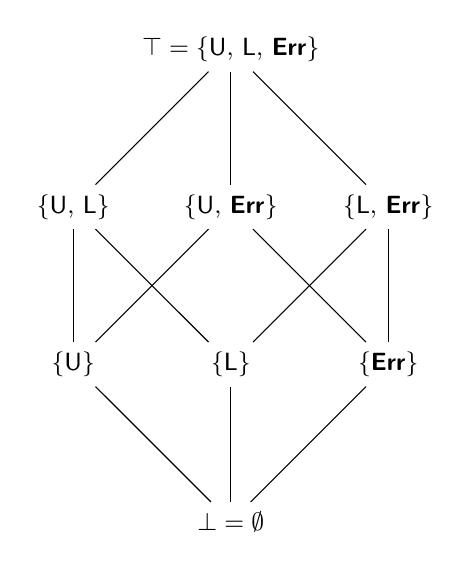
\begin{tikzpicture}[font=\small]
      \node (N_3) at (0,0) {$\top = \{\text{\textsf{U}},\, \text{\textsf{L}},\, \text{\textbf{\textsf{Err}}}\}$};

      \node (N_2A) at (-2,-2) {$\{\text{\textsf{U}},\, \text{\textsf{L}}\}$}
	edge node {} (N_3);
      \node (N_2B) at (0,-2) {$\{\text{\textsf{U}},\, \text{\textbf{\textsf{Err}}}\}$}
	edge node {} (N_3);
      \node (N_2C) at (2,-2) {$\{\text{\textsf{L}},\, \text{\textbf{\textsf{Err}}}\}$}
	edge node {} (N_3);

      \node (N_1A) at (-2,-4) {$\{\text{\textsf{U}}\}$}
	edge node {} (N_2A)
	edge node {} (N_2B);
      \node (N_1B) at (0,-4) {$\{\text{\textsf{L}}\}$}
	edge node {} (N_2A)
	edge node {} (N_2C);
      \node (N_1C) at (2,-4) {$\{\text{\textbf{\textsf{Err}}}\}$}
	edge node {} (N_2B)
	edge node {} (N_2C);

      \node (N_0) at (0,-6) {$\bot=\emptyset$}
	edge node {} (N_1A)
	edge node {} (N_1B)
	edge node {} (N_1C);
    \end{tikzpicture}}
  \end{tabular}
  \end{center}

\end{frame}

\begin{frame}
  \frametitle{Model Checking Issue}

  \begin{textblock*}{0.56\textwidth}(0.26\textwidth,1cm)
  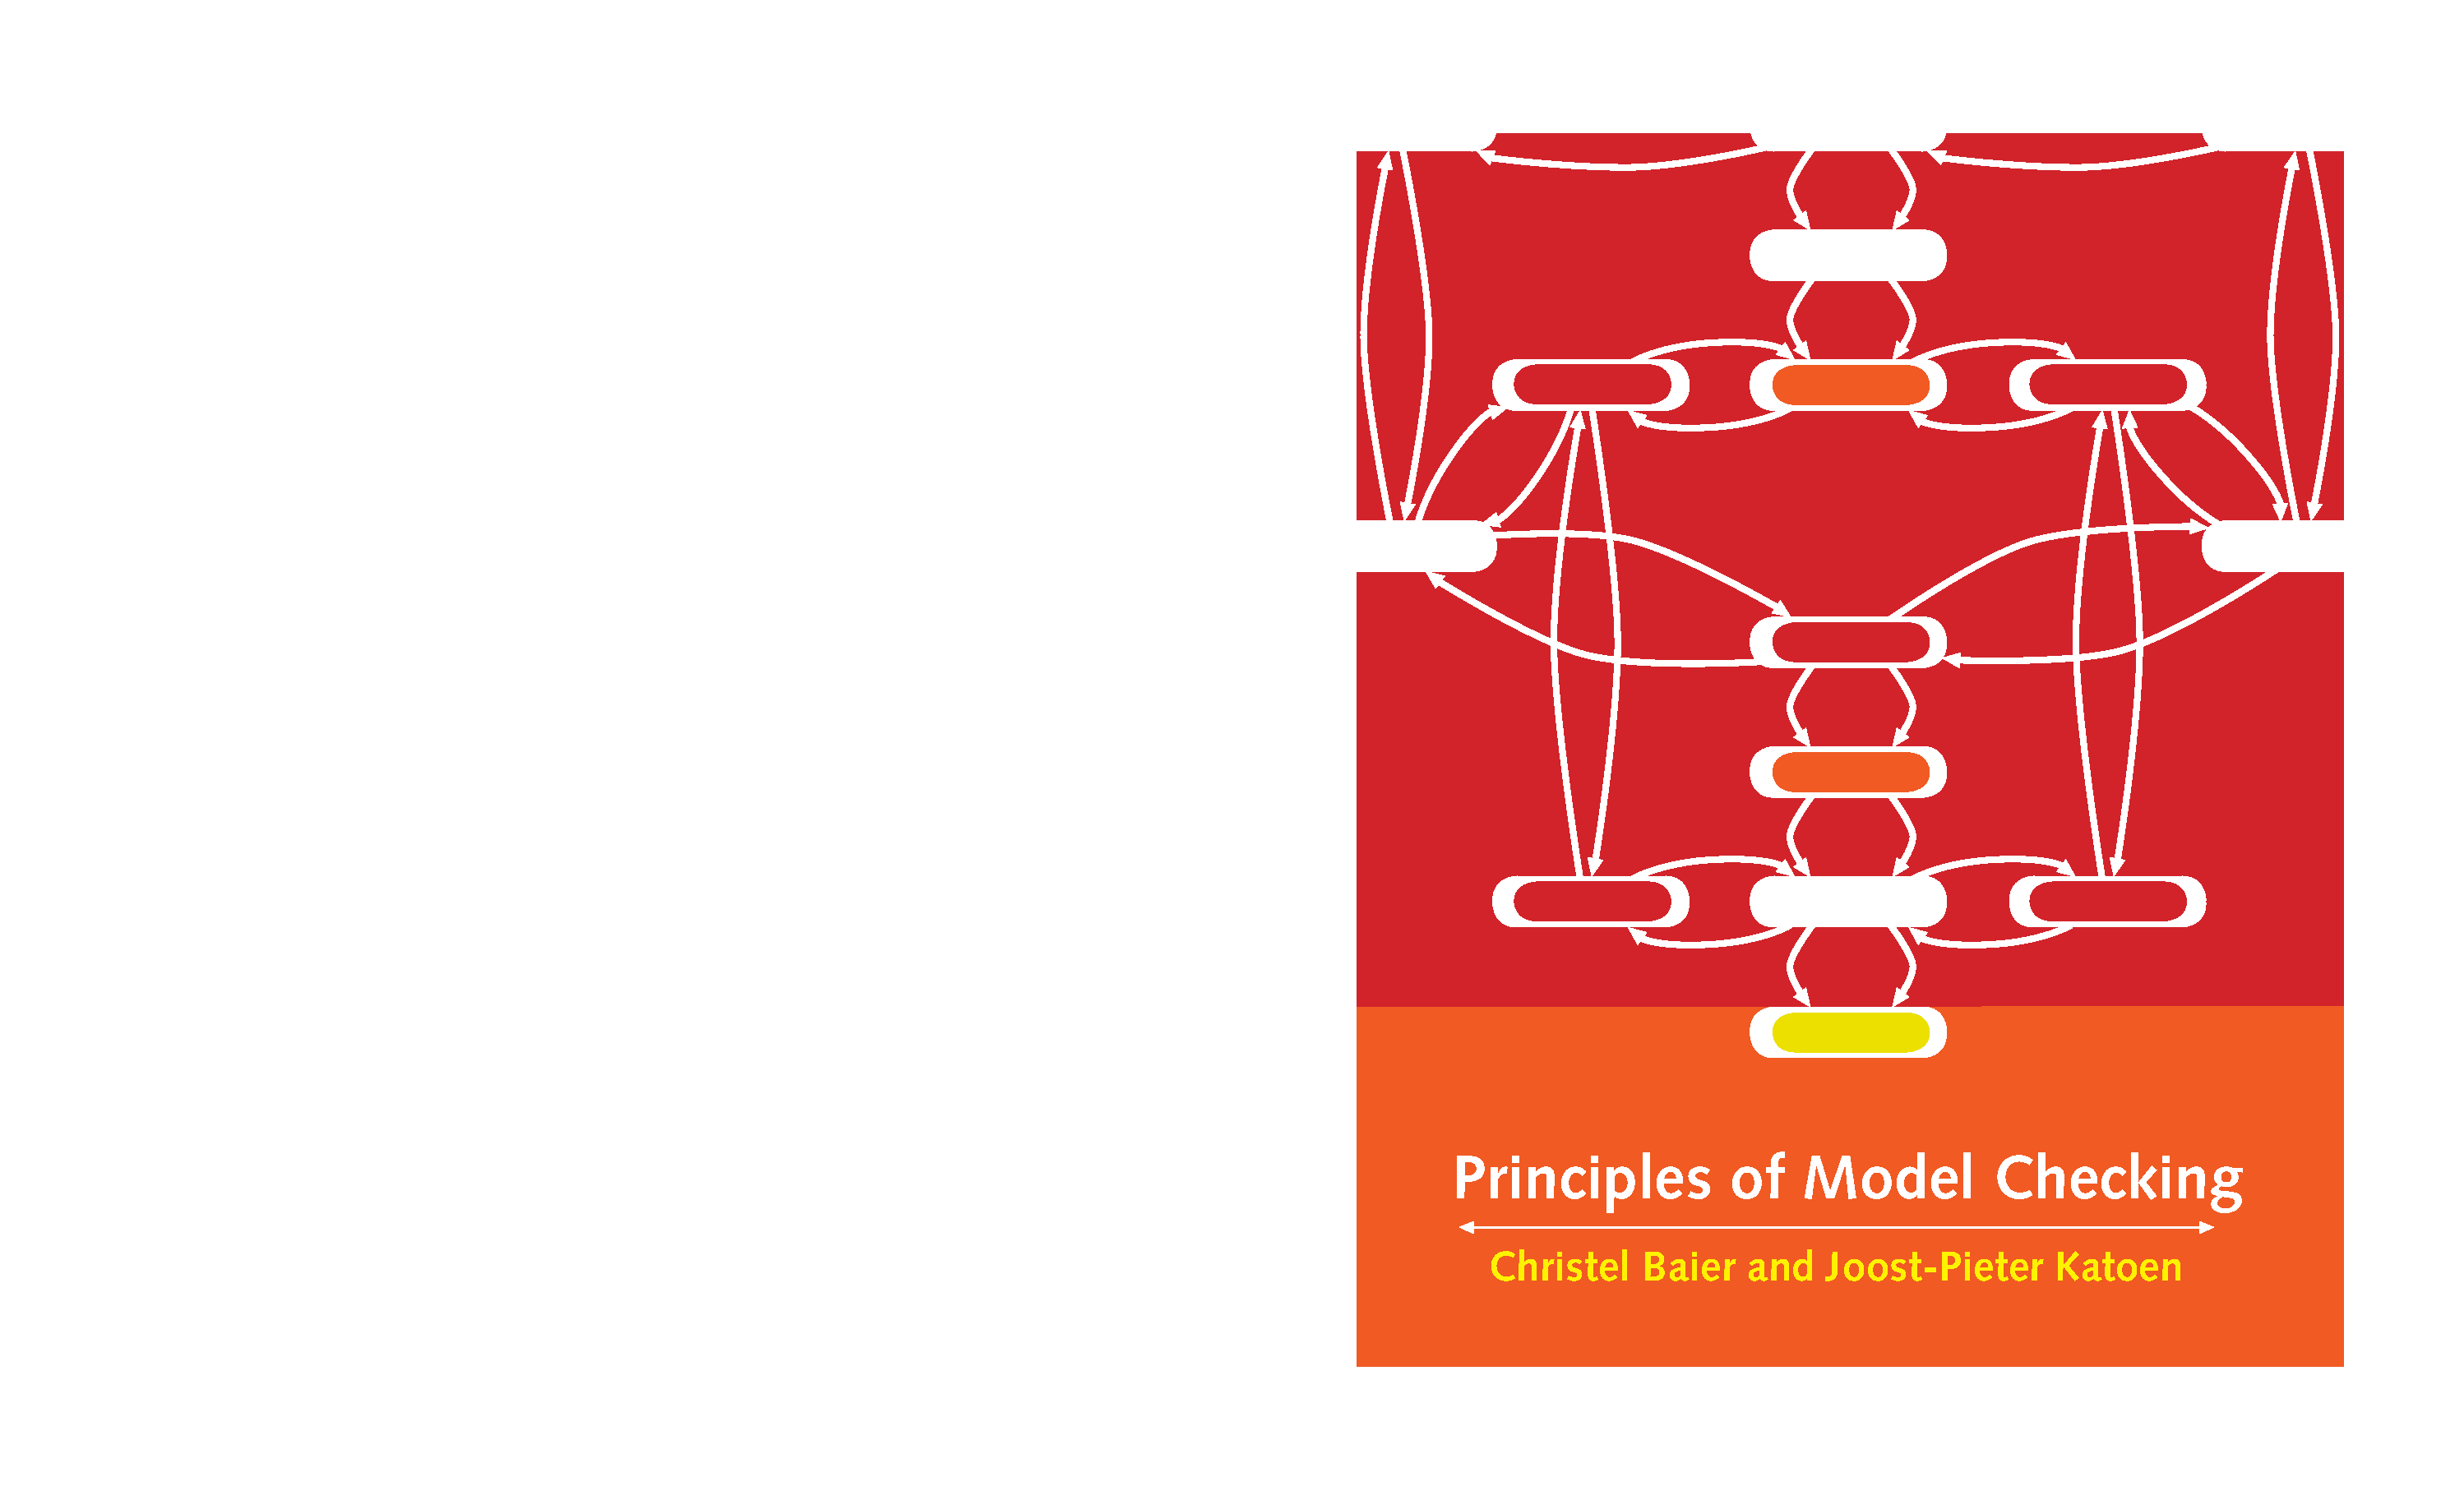
\includegraphics[width=\textwidth]{principles_of_mc}
  \end{textblock*}

  \begin{textblock*}{12cm}(0.3cm,1.1cm)
  \only<2>{
  \colorbox[rgb]{0.972 0.925 0.76}{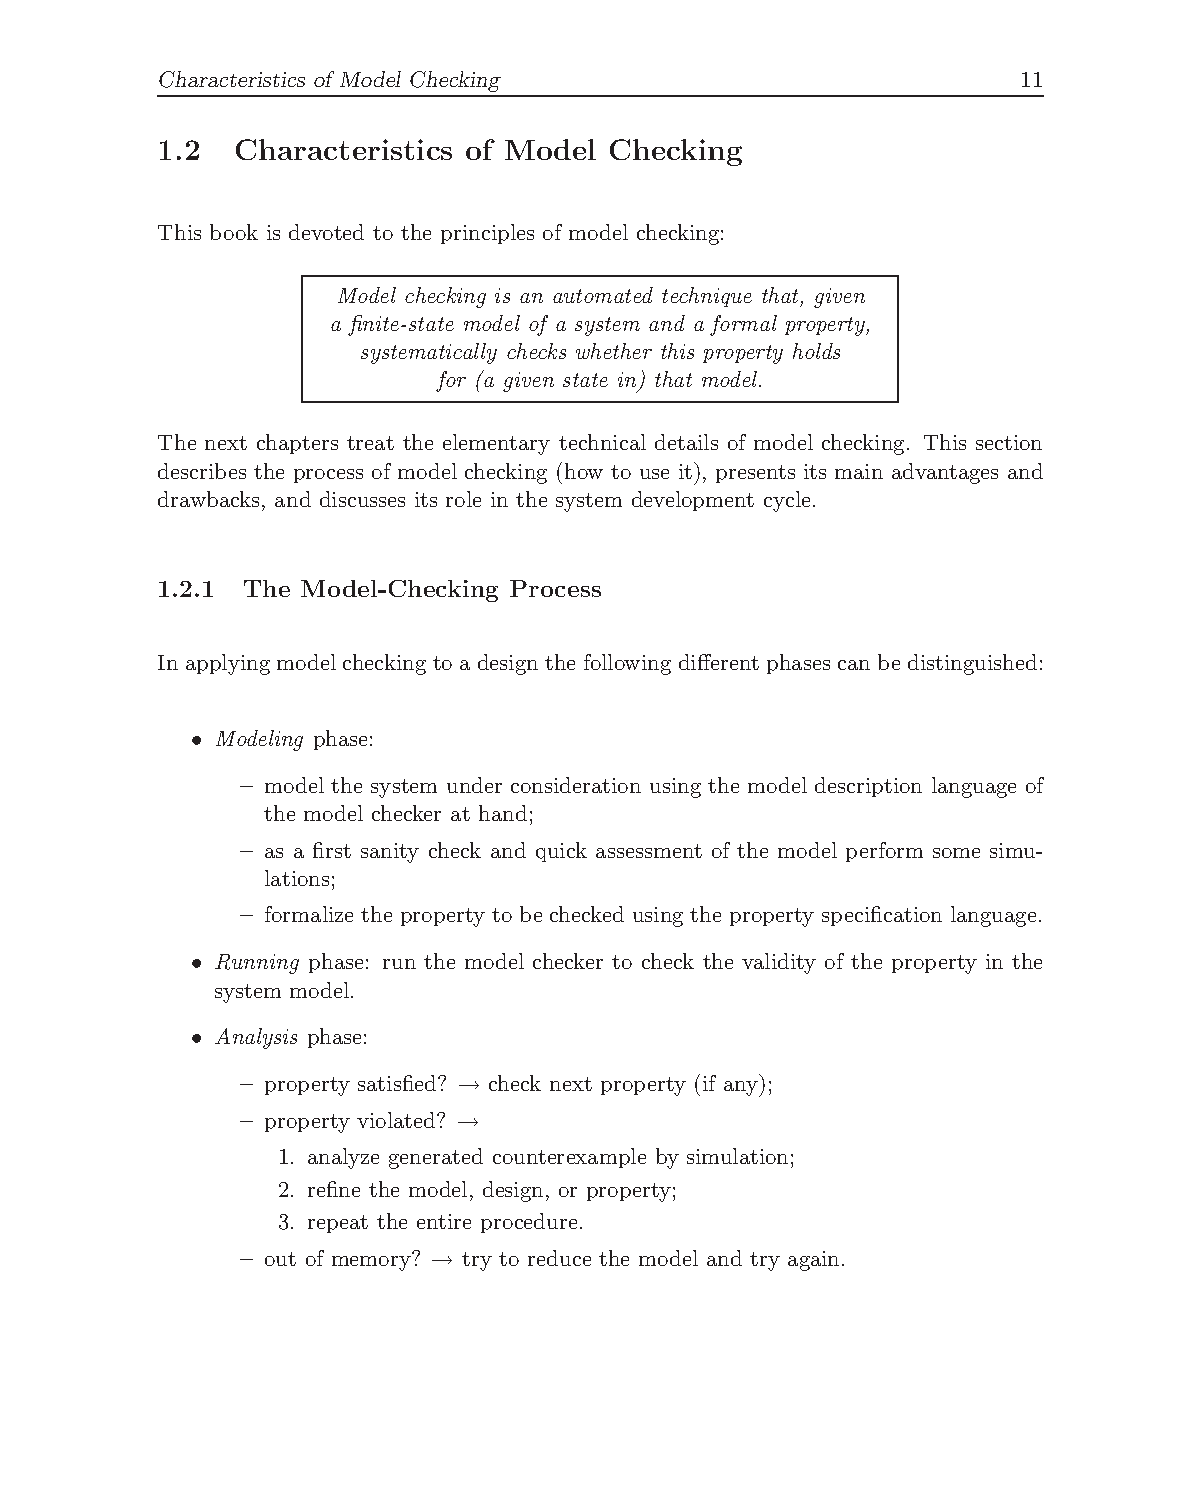
\includegraphics[width=\textwidth,clip,trim=2.65cm 17.85cm 4.9cm 1.1cm]{principles_of_mc_1}}}
  \end{textblock*}

\end{frame}

\setcounter{framenumber}{\value{finalframe}}

\end{document}
